\subsection{Disk performance}

\subsubsection{HDD}

We can calculate some performance metrics related to the types of delay of HDD (page \pageref{four types of hdd delay}).
\begin{itemize}
    \item \definition{Full Rotation Delay} $R$ is:
    \begin{equation}
        R = \dfrac{1}{\texttt{DiskRPM}}
    \end{equation}
    And in seconds:
    \begin{equation}
        R_{\text{sec}} = 60 \times R
    \end{equation}
    From the $R_{\text{sec}}$ we can also calculate the \definition{total rotation average}:
    \begin{equation}
        T_{\text{rotation AVG}} = \dfrac{R_{\text{sec}}}{2}
    \end{equation}

    \item \definition{Seek Time}, the \textbf{time to move the head to a different track}, which is divided into several phases:
    \begin{itemize}
        \item Acceleration
        \item Coasting (constant speed)
        \item Deceleration
        \item Settling
    \end{itemize}
    The $T_{\text{seek}}$ modelling considers a linear dependency with the distance. Also, the \definition{seek average} is:
    \begin{equation}
        T_{\text{seek AVG}} = \dfrac{T_{\text{seek MAX}}}{3}
    \end{equation}

    \item \definition{Transfer time}. It is the \textbf{time that data is either read from or written to the surface}. It \textbf{includes} the time the \textbf{head needs to pass on the sectors} and the \textbf{I/O transfer}. The \definition{Controller Overhead} is the \textbf{buffer management} (data transfer) and \textbf{interrupt sending time}.

    Transfer time and Controller Overhead are together because they are required to calculate some interesting metrics.
    \begin{itemize}
        \item \definition{Service Time} $T_{\text{I/O}}$
        \begin{equation}
            T_{\text{I/O}} = T_{\text{seek}} + T_{\text{rotation}} + T_{\text{transfer}} + T_{\text{overhead}}
        \end{equation}

        \item \definition{Response Time}
        \begin{equation}
            T_{\text{queue}} + T_{\text{I/O}}
        \end{equation}
        Where $T_{\text{queue}}$ depends on queue-length, resource utilization, mean and variance of disk service time and request arrival distribution.
    \end{itemize}
    \newpage
    \begin{figure}[!htp]
        \centering
        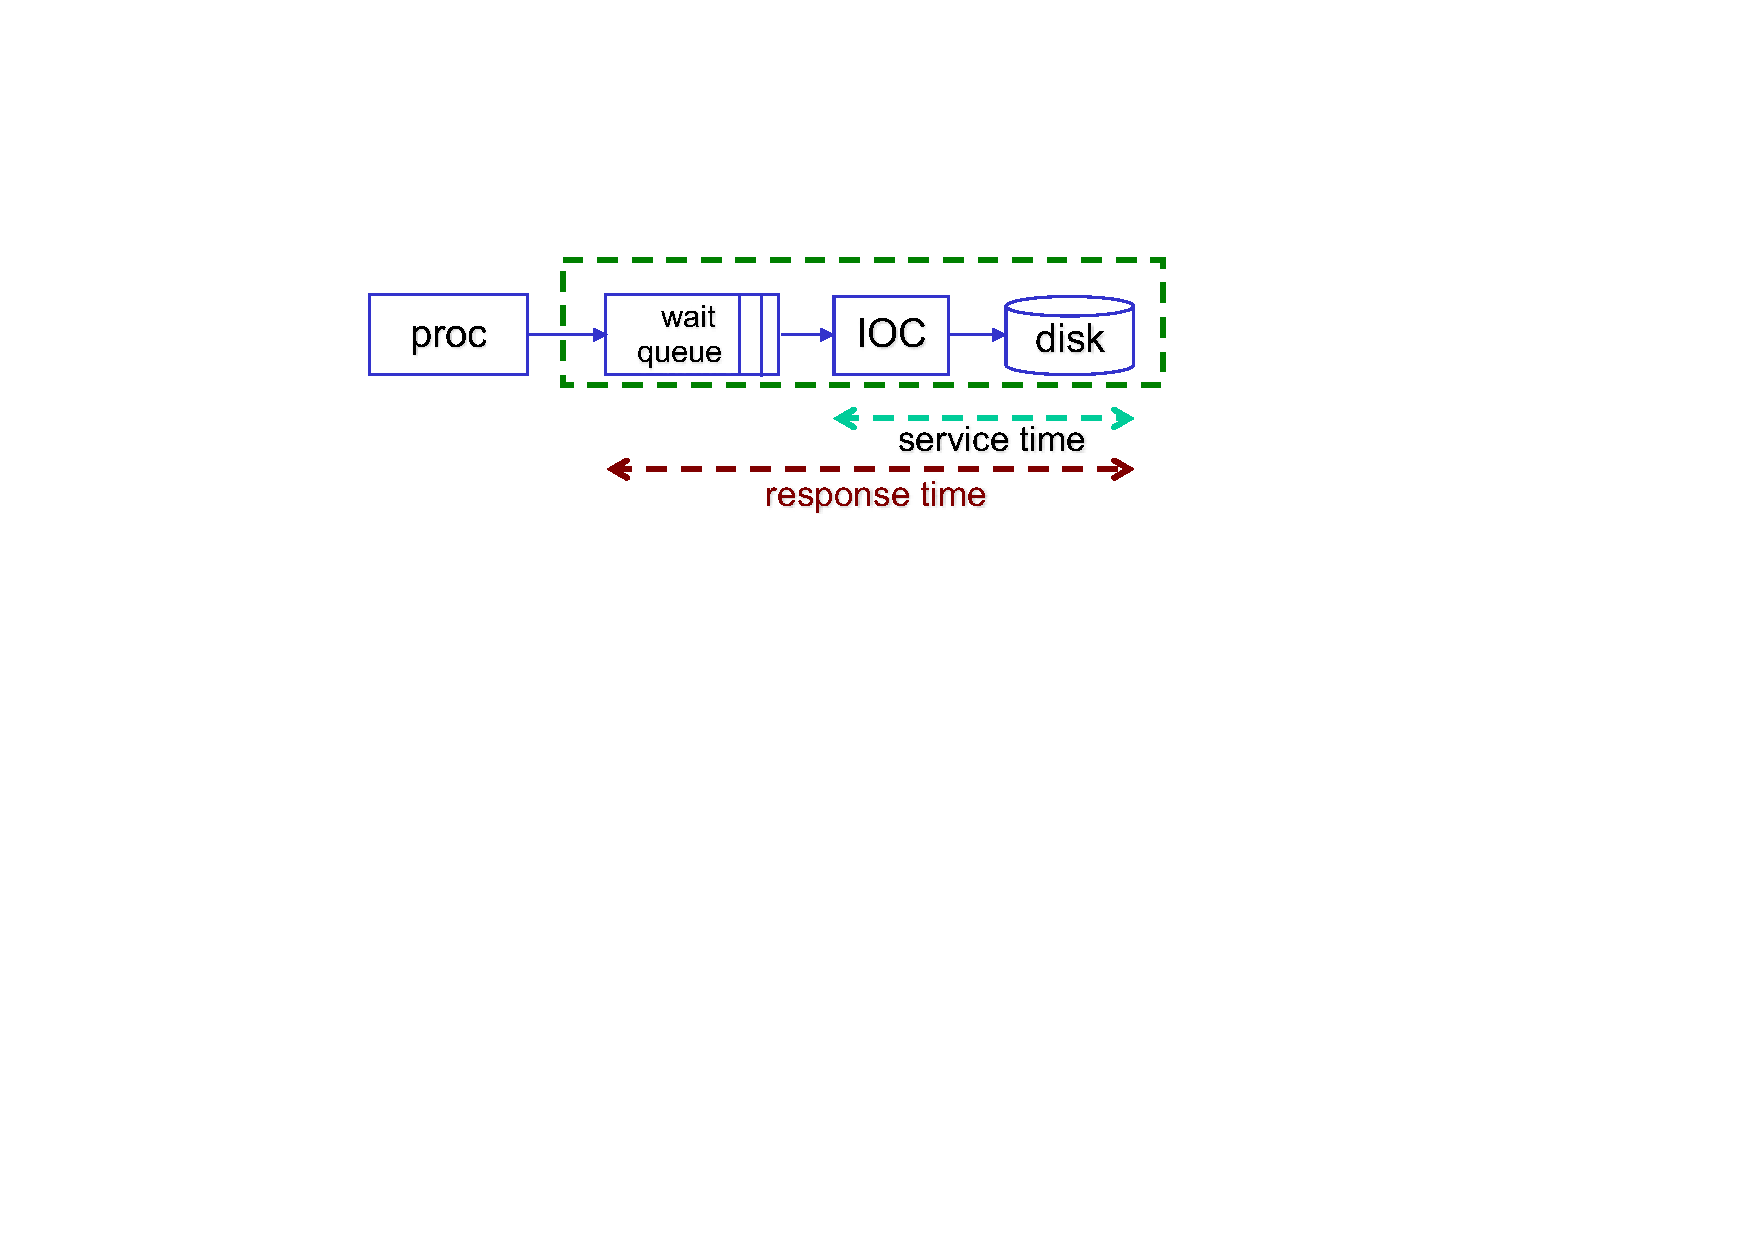
\includegraphics[width=.7\textwidth]{img/performance-hdd-1.pdf}
        \caption{Service and response time.}
    \end{figure}
\end{itemize}